\documentclass[fleqn, a4paper, 12pt, twoside]{article}
\usepackage{exsheets}
\usepackage{amsmath, amssymb, amsthm} %standard AMS packages
\usepackage{marginnote} %marginnotes
\usepackage{gensymb} %miscellaneous symbols
\usepackage{commath} %differential symbols
\usepackage{xcolor} %colours
\usepackage{cancel} %cancelling terms
\usepackage{siunitx} %formatting units
\usepackage{tikz, pgfplots} %diagrams
	\usetikzlibrary{calc, hobby, patterns, intersections}
\usepackage{graphicx} %inserting graphics
\usepackage{epstopdf}
\usepackage{hyperref} %hyperlinks
\usepackage{datetime} %date and time
\usepackage{ulem} %underline for \emph{}
\usepackage{xfrac} %inline fractions
\usepackage{enumerate} %numbered lists
\usepackage{float} %inserting floats
\usepackage{circuitikz} %circuit diagrams

\newcommand\numberthis{\addtocounter{equation}{1}\tag{\theequation}} %adds numbers to specific equations in non-numbered list of equations

\newcommand{\AxisRotator}[1][rotate=0]{
	\tikz [x=0.25cm,y=0.60cm,line width=.2ex,-stealth,#1] \draw (0,0) arc (-150:150:1 and 1);%
} %rotation symbols on axes

\theoremstyle{definition}
\newtheorem{example}{Example}
\newtheorem{definition}{Definition}

\theoremstyle{theorem}
\newtheorem{theorem}{Theorem}

\newcommand{\curl}{\mathrm{curl\,}}

\makeatletter
\@addtoreset{section}{part} %resets section numbers in new part
\makeatother

\newcommand\blfootnote[1]{%
	\begingroup
	\renewcommand\thefootnote{}\footnote{#1}%
	\addtocounter{footnote}{-1}%
	\endgroup
}

\SetupExSheets{solution/print = true}

%opening
\title{Physics 2}
\author{Aakash Jog}
\date{2014-15}

\begin{document}

\maketitle
%\setlength{\mathindent}{0pt}

\blfootnote
{	
	\begin{figure}[H]
		
\includegraphics[height = 12pt]{cc.eps}
		\includegraphics[height = 12pt]{by.eps}
		\includegraphics[height = 12pt]{nc.eps}
		\includegraphics[height = 12pt]{sa.eps}
	\end{figure}
	This work is licensed under the Creative Commons Attribution-NonCommercial-ShareAlike 4.0 International License. To view a copy of this license, visit \url{http://creativecommons.org/licenses/by-nc-sa/4.0/}.
}

\tableofcontents

\newpage
\section{Lecturer Information}

\textbf{Dr. Erez Pyetan}\\
~\\
Office: Sharet 325\\
Telephone: 7565\\
E-mail: erezpyet@mail.tau.ac.il\\

\section{Textbooks}

\begin{enumerate}
	\item D. Halliday, R. Resnick, and K. S. Krane: \textit{Physics}, 5th edition, vol. 2 (Wiley)
	\item D.J. Griffiths: \textit{Introduction to Electrodynamics}
\end{enumerate}

\newpage
\part{Electrostatics}

\section{Coulomb's Law}

The force between two charged particles is directly proportional to the product of the charges of the particles, and inversely proportional to the square of the distance between them.
\begin{align*}
	F &\propto \dfrac{q_1 q_2}{r^2}\\
	F &= k \dfrac{q_1 q_2}{r^2}\\
	&= \dfrac{1}{4 \pi \varepsilon_0} \cdot \dfrac{q_1 q_2}{r^2}
\end{align*}
The constant of proportionality is $k = 8.99 \times 10^9 \si{\newton\metre\squared\per\coulomb\squared}$.\\
$\varepsilon_0 = 8.8541878162 \times 10^{-12} \si{\coulomb\squared\per\newton\per\metre\squared}$ is called the permittivity of free space.\\
In vector notation,
\begin{align*}
	\overrightarrow{F_{2 1}} &= \dfrac{1}{4 \pi \varepsilon_0} \dfrac{q_1 q_2}{{r_{1 2}}^2} \hat{r_{1 2}}
\end{align*}
~\\
Charge is defined according to this law.\\

\begin{question}
	A charge $q$ is placed at the origin. A charge $-2q$ is placed at 1 \si{\metre} from it, in the $x$ direction. Find a point on the $y$-axis where the total force acting on a charge $q'$ will be parallel to the $x$-axis.\\
\end{question}

\begin{solution}
	\begin{figure}[H]
		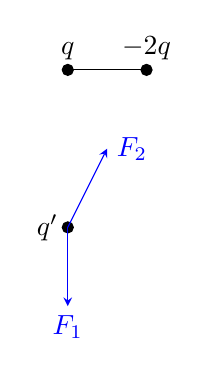
\begin{tikzpicture}
			\def\y{-2};
			\def\F{1};
			
			\coordinate (q) at (0,0);
			\coordinate (-2q) at (1,0);
			\coordinate (q') at (0,\y);
			
			\filldraw (q) circle [radius = 2pt] node [above] {$q$};
			\filldraw (-2q) circle [radius = 2pt] node [above] {$-2q$};
			\filldraw (q') circle [radius = 2pt] node [left] {$q'$};
			
			\draw (q) -- (-2q);
			
			\begin{scope}[blue, -stealth]
				\draw (q') -- ++(-90:\F) node [below] {$F_1$};
				\draw (q') -- ($ (q') ! 0.5 ! (-2q) $) node [right] {$F_2$};
			\end{scope}
		\end{tikzpicture}
	\end{figure}
	For the net force to be in the $x$ direction, the components of $F_1$ and $F_2$ in the $y$ direction must cancel each other out.
	\begin{align*}
		F_1 &= F_2 \sin \theta\\
		\therefore \cancel{k} \cdot \dfrac{(\cancel{q'})(-2\cancel{q})}{y^2 + 1} \cdot \dfrac{y}{\sqrt{y^2 + 1}} &= \cancel{k} \cdot \dfrac{(\cancel{q})(\cancel{q'})}{y^2}\\
		\therefore \dfrac{-2y}{(y^2 + 1)^{\sfrac{3}{2}}} &= \dfrac{1}{y^2}\\
		\therefore y &= \pm \sqrt{\dfrac{1}{2^{\sfrac{2}{3}}- 1}}
	\end{align*}
\end{solution}

\begin{question}
	A rod of length $L$ has a uniformly distributed charge $Q$, with line charge density $\lambda = \dfrac{Q}{L}$. A point charge $q$ is kept at a distance $x$ as shown.
	\begin{figure}[H]
		\begin{tikzpicture}
			\def\L{5};
			\def\x{10};
			
			\coordinate (q) at (\x,0);
			
			\draw [ultra thick] (0,\L/2) -- (0,-\L/2);
			
			\filldraw (q) circle [radius = 2pt] node [right] {$q$};
			
			\begin{scope}[|<->|]
				\draw [xshift = -20] (0,\L/2) -- (0,-\L/2) node [midway, fill = white] {$L$};
				\draw [xshift = -10] (0,\L/2) -- (0,0) node [midway, fill = white] {$\dfrac{L}{2}$};
			\end{scope}
		\end{tikzpicture}
	\end{figure}
\end{question}

\begin{solution}
	\begin{figure}[H]
		\begin{tikzpicture}
			\def\L{5};
			\def\x{10};
			\def\y{0.75*\L/2};
			\def\dy{0.1*\y};
			
			\coordinate (q) at (\x,0);
			\coordinate (dq) at (0, {\y + (\dy/2)});
			
			\draw [ultra thick] (0,\L/2) -- (0,-\L/2);
			
			\filldraw (q) circle [radius = 2pt] node [above] {$q$};
			
			\begin{scope}[dashed]
				\draw (q) -- (dq) node [midway, fill = white] {$r = \sqrt{x^2 + y^2}$};
				\draw (q) -- (0,0);
			\end{scope}
			
			\begin{scope}[red, -stealth]
				\draw (q) -- ($(q) ! -1cm ! (dq)$) node [below right] {$\dif F$};
			\end{scope}
			
			\draw [|<->|, yshift = -10] (0,0) -- (\x,0) node [midway, fill = white] {$x$};
			\draw [|<->|, xshift = -10] (0,0) -- (0,\y) node [midway, fill = white] {$y$};
			
			\draw [|-|, xshift = -10] (0,\y) -- ++(0,\dy) node [midway, left] {$\dif y$};
		\end{tikzpicture}
	\end{figure}
	The $y$ components of the forces of the elemental charges at $y$ and $-y$ on $q$ are cancelled out. Therefore, the net force is in the $x$ direction only.
	\begin{align*}
		\dif F &= k \dfrac{(\dif Q) (q)}{r^2}\\
		\dif F_x &= \dif F \cos \theta\\
		&= k \dfrac{(\dif Q) (q)}{r^2} \cos \theta\\
		&= k \dfrac{(\lambda \dif y) (q)}{x^2 + y^2} \dfrac{x}{\sqrt{x^2 + y^2}}\\
		&= k \lambda q x \dfrac{\dif y}{(x^2 + y^2)^{\sfrac{3}{2}}}\\
		\therefore \overrightarrow{F} &= \hat{x} \int \dif F_x\\
		&= \hat{k} \lambda q x \int\limits_{-\sfrac{L}{2}}^{\sfrac{L}{2}} \dfrac{\dif y}{(x^2 + y^2)^{\sfrac{3}{2}}}
	\end{align*}
		Substituting $y = x \tan \theta$ and $\dif y = x \sec^2 \theta \dif \theta$
	\begin{align*}
		\overrightarrow{F} &= \hat{x} \lambda q k x \int\limits_{-\theta_0}^{\theta_0} \dfrac{1}{x^2} \cos \theta \dif \theta\\
		&= \hat{x} \dfrac{\lambda q k}{x} \int\limits_{-\theta_0}^{\theta_0} \cos \theta \dif \theta
	\end{align*}
		Therefore,
	\begin{align*}
		\overrightarrow{F} &= \hat{x} \dfrac{2 \lambda q k}{x} \sin \theta_0\\
		&= \hat{x} \dfrac{2 \lambda q k}{x} \dfrac{\dfrac{L}{2}}{\left( \left( \dfrac{L}{2} \right)^2 + x^2 \right)^{\sfrac{1}{2}}}\\
		&= \hat{x} \dfrac{2 \left( \dfrac{Q}{L} \right) q k}{x} \cdot  \dfrac{\dfrac{L}{2}}{\left( \left( \dfrac{L}{2} \right)^2 + x^2 \right)^{\sfrac{1}{2}}}\\
		&= k \dfrac{Q q}{x \left( \left( \dfrac{L}{2} \right)^2 + x^2 \right)^{\sfrac{1}{2}}} \hat{x}
	\end{align*}
\end{solution}

\begin{question}
	A point charge $q$ is kept at a distance $z$ above a ring of radius $R$ charged with $Q = 2 \pi R \lambda$, where $\lambda$ is the linear charge density. Find the force acting on $q$.
\end{question}

\begin{solution}
	\begin{figure}[H]
		\begin{tikzpicture}
			\def\R{3};
			\def\z{5};
			
			\coordinate (q) at (0,\z);
			\coordinate (dQ) at (-\R,0);
			
			\draw (0,0) circle [x radius = \R, y radius = 0.4*\R];
			
			\filldraw (q) circle [radius = 2pt] node [above] {$q$};
			
			\begin{scope}[dashed]
				\draw (0,0) -- (q);
				\draw (0,0) -- (dQ);
				\draw (q) -- (dQ) node [midway, fill = white] {$\sqrt{z^2 + R^2}$};
			\end{scope}
		\end{tikzpicture}
	\end{figure}
	Due to the symmetry of the ring, the net force acting on $q$ is in the $z$ direction only.
	\begin{align*}
		\dif F_z &= \dif F \cos \theta\\
		&= k \dfrac{(\dif Q) (q)}{z^2 + R^2} \cos \theta\\
		&= k \dfrac{(\dif Q) (q)}{z^2 + R^2} \dfrac{z}{\sqrt{z^2 + R^2}}\\
		&= k q z \dfrac{\dif Q}{\left( z^2 + R^2 \right)^{\sfrac{3}{2}}}\\
		\therefore \overrightarrow{F} &= \hat{z} \int \dif F_z\\
		&= \hat{z} k q z \dfrac{1}{\left( z^2 + R^2 \right)^{\sfrac{3}{2}}} \int\limits_{0}^{Q} \dif Q\\
		&= k \dfrac{Q q z}{\left( z^2 + R^2 \right)^{\sfrac{3}{2}}} \overrightarrow{z}
	\end{align*}
\end{solution}

\begin{question}
	A point charge $q$ is kept at a distance $z$ above a disk of radius $R$ charged with $Q = \pi R^2 \sigma$, where $\sigma$ is the surface charge density. Find the force acting on $q$.
\end{question}

\begin{solution}
	The disk can be considered to be made up of elemental rings, with radii varying from $0$ to $R$.\\
	Therefore,
	\begin{align*}
		\dif \overrightarrow{F} &= k \dfrac{q Q_{\textnormal{ring}}}{\left( z^2 + R^2 \right)^{\sfrac{3}{2}}} \hat{z}\\
		&= k \dfrac{q (\sigma \cdot 2 \pi r \cdot \dif r)}{\left( z^2 + R^2 \right)^{\sfrac{3}{2}}} z \hat{z}
	\end{align*}
	Hence,
	\begin{align*}
		\overrightarrow{F} &= \int \dif\overrightarrow{F}\\
		&= \hat{z} \int\limits_{0}^{R} k \dfrac{q \sigma \cdot 2 \pi r z \cdot \dif r}{\left( z^2 + R^2 \right)^{\sfrac{3}{2}}}\\
		&= 2 k z q \sigma \pi \left( \dfrac{1}{|z|} - \dfrac{1}{\sqrt{z^2 + R^2}} \right)\hat{z}
	\end{align*}
	If $z << R$, i.e. for an infinite sheet,
	\begin{align*}
		F &= 2 q \sigma \pi k 
	\end{align*}
\end{solution}

\end{document}